\documentclass[conference]{IEEEtran}
\IEEEoverridecommandlockouts
\usepackage{cite}
\usepackage{amsmath,amssymb,amsfonts}
\usepackage{algorithmic}
\usepackage{graphicx}
\usepackage{textcomp}
\usepackage{xcolor}
\usepackage{booktabs}
\usepackage{algorithm}
\usepackage{listings}
\usepackage{url}
\usepackage{tabularx}
\usepackage{multirow}
\usepackage{tikz}
\usetikzlibrary{shapes,arrows,positioning}
\usepackage{pgfplots}
\pgfplotsset{compat=1.18}

\def\BibTeX{{\rm B\kern-.05em{\sc i\kern-.025em b}\kern-.08em
    T\kern-.1667em\lower.7ex\hbox{E}\kern-.125emX}}

\lstset{
  language=Python,
  basicstyle=\ttfamily\footnotesize,
  keywordstyle=\color{blue},
  stringstyle=\color{red},
  commentstyle=\color{green!60!black},
  numbers=left,
  numberstyle=\tiny\color{gray},
  stepnumber=1,
  breaklines=true,
  frame=single,
  showstringspaces=false,
  captionpos=b
}

\begin{document}

\title{Carbon-Track Transpiler: AST-Driven Source-to-Source Optimization for Energy-Efficient Software Execution}

\author{
\IEEEauthorblockN{Shweta Tiwaskar}
\IEEEauthorblockA{\textit{Department of Computer Engineering} \\
\textit{Vishwakarma Institute of Technology}\\
Pune, India \\
shweta.tiwaskar@vit.edu}
\and
\IEEEauthorblockN{Sahil Jadhav}
\IEEEauthorblockA{\textit{Department of Computer Engineering} \\
\textit{Vishwakarma Institute of Technology}\\
Pune, India \\
sahil.jadhav241@vit.edu}
\and
\IEEEauthorblockN{Kushal Chaudhari}
\IEEEauthorblockA{\textit{Department of Computer Engineering} \\
\textit{Vishwakarma Institute of Technology}\\
Pune, India \\
kushal.chaudhari24@vit.edu}
\and
\IEEEauthorblockN{Shiv Wagh}
\IEEEauthorblockA{\textit{Department of Computer Engineering} \\
\textit{Vishwakarma Institute of Technology}\\
Pune, India \\
shiv.wagh24@vit.edu}
\and
\IEEEauthorblockN{Shreyash Chilip}
\IEEEauthorblockA{\textit{Department of Computer Engineering} \\
\textit{Vishwakarma Institute of Technology}\\
Pune, India \\
shreyash.chilip24@vit.edu}
}

\maketitle

%% ─────────────────────────────────────────────────────────────────────────────
\begin{abstract}
The rapid proliferation of cloud computing, artificial intelligence, and
hyperscale web services has catalyzed an exponential increase in global
energy consumption attributable to the Information and Communication
Technology (ICT) sector.  Although hardware efficiency has improved
steadily over the past two decades, the software driving modern
infrastructure frequently remains unoptimized for energy consumption.
Current software-engineering practices prioritize delivery velocity and
functional correctness, systematically overlooking the computational
inefficiency and resulting environmental footprint of deployed codebases.
Dynamically typed, interpreted languages such as Python are ubiquitous in
data science, machine learning, and web back-ends, yet they carry
significant runtime overhead that directly translates to elevated electricity
consumption.  Bridging the gap between compiler theory and environmental
responsibility, this paper introduces the \textbf{Carbon-Track Transpiler
(CTT)}, a novel Abstract Syntax Tree (AST)-driven, source-to-source
optimization framework.  CTT automatically parses, statically analyzes, and
rewrites unoptimized Python source files, producing functionally equivalent
outputs whose structural changes minimize CPU instruction counts, memory
access operations, and total wall-clock execution time.  Compiler-level
techniques---constant folding, strength reduction, dead-code elimination,
loop fusion, loop-append-to-comprehension conversion, and list-to-set
membership promotion---are applied entirely at the source level, preserving
human readability and developer transparency.  Integrated seamlessly with
the CodeCarbon library, CTT's Carbon Auditing Engine measures empirical
energy savings (kWh) and carbon-equivalent emissions ($\mathrm{kgCO_2eq}$)
for both the original and transpiled scripts.  Empirical evaluation across
eight diverse algorithmic and data-engineering benchmarks demonstrates an
average execution-time reduction of \textbf{15\%--40\%}, an average energy
saving of \textbf{up to 35\%}, and a commensurate reduction in carbon
emissions.  These results establish CTT as a practical, automated pipeline
for operationalizing Green Software Engineering at the developer's workstation
and inside CI/CD pipelines.
\end{abstract}

\begin{IEEEkeywords}
Green Computing, Abstract Syntax Tree, Source-to-Source Compilation,
Sustainable Software Engineering, Energy-Efficient Code, Static Analysis,
Carbon Tracking, Python Optimization, Compiler Transformations
\end{IEEEkeywords}

%% ─────────────────────────────────────────────────────────────────────────────
\section{Introduction}

The global digital economy runs on software.  From the data centers that
host cloud workloads to the mobile devices that connect billions of users,
software-defined computations dictate the magnitude and pattern of electrical
energy consumed by modern computing infrastructure.  Data centers alone are
estimated to account for approximately 1\%--2\% of global electricity use,
while the broader ICT ecosystem---including communication networks and
end-user devices---accounts for 5\%--9\% of total electricity demand
\cite{ref1}.  With the relentless growth of machine-learning workloads, large
language models, and real-time analytics platforms, these figures are projected
to increase substantially over the coming decade.

Historically, efforts to curtail the energy footprint of computing
concentrated on hardware innovation: improving processor microarchitectures,
adopting more efficient memory technologies, and optimizing data-center Power
Usage Effectiveness (PUE) \cite{ref4}.  These hardware-centric strategies have
yielded significant dividends.  However, they address only one side of the
energy equation.  Software is the ultimate governor of hardware behavior: it
determines how many CPU instructions are issued, how frequently the memory
hierarchy is accessed, and how long the processor spends in high-power active
states versus low-power idle states.  Poorly structured code mandates
unnecessary computational work that hardware efficiency gains cannot fully
compensate for.

This problem is particularly severe in Python-dominated workloads.  Python's
dynamically typed, interpreted execution model makes it extraordinarily
productive for developers, but at the cost of substantial runtime overhead.
The Python Virtual Machine (PVM) must perform dynamic type dispatch, reference
counting, and bytecode interpretation for every operation, amplifying the
energy cost of suboptimal coding patterns.  Empirical studies have shown that
equivalent computations can consume an order of magnitude more energy in Python
than in a compiled language such as C \cite{ref7}.  Given that Python has
become the dominant language for data science, AI research, and backend
services, addressing its energy profile is a matter of practical urgency.

Contemporary static-analysis tools and linters (e.g., Pylint, Flake8,
Bandit) focus primarily on correctness, style, and security; they are
largely blind to the energy implications of specific code structures
\cite{ref6}.  Runtime approaches such as Just-In-Time compilation (e.g., PyPy,
Numba) can improve performance but alter the execution environment, introduce
warmup latency, and may be incompatible with C-extension libraries that are
ubiquitous in scientific Python.  There is, therefore, a clear and compelling
need for a tool that (a) operates statically at the source level, (b) applies
compiler-grade optimizations transparently, and (c) quantifies the resulting
energy and carbon savings empirically.

The \textbf{Carbon-Track Transpiler (CTT)} addresses this need.  CTT is an
automated framework built on Python's native \texttt{ast} module.  It reads
an unoptimized Python script, traverses the resulting Abstract Syntax Tree
(AST), applies a suite of semantics-preserving transformation rules, and
unparses the optimized AST back into readable Python source code.  Crucially,
it pairs every transformation with an empirical Carbon Audit that uses the
CodeCarbon library \cite{ref9} to measure hardware-level energy consumption
via Intel RAPL (Running Average Power Limit) counters, ultimately reporting
energy savings in kWh and $\mathrm{kgCO_2eq}$.

The principal contributions of this paper are:
\begin{itemize}
  \item A comprehensive taxonomy of ``energy-smell'' patterns in Python
        amenable to safe, static AST refactoring.
  \item A modular, extensible AST-based source-to-source transpilation
        pipeline implementing six optimization passes.
  \item An integrated, empirical Carbon Auditing Engine that correlates
        structural transformations with hardware-measured energy savings.
  \item Empirical evaluation across eight benchmarks demonstrating up to
        40\% execution-time reduction and 35\% energy saving.
  \item A discussion of the safety guarantees, trade-offs, and limitations
        of static optimization in a dynamically typed language.
\end{itemize}

The remainder of the paper is organized as follows.  Section~II provides
background on Green Computing, ASTs, source-to-source optimization, and
carbon tracking.  Section~III reviews related work.  Section~IV compares
CTT against existing tools.  Section~V describes the methodology and system
architecture.  Section~VI presents the formal algorithms.  Section~VII
illustrates concrete input--output transformations.  Section~VIII describes
the experimental setup.  Section~IX presents and discusses results.
Sections~X--XII address impact, limitations, and future scope.
Section~XIII concludes the paper.

%% ─────────────────────────────────────────────────────────────────────────────
\section{Background}

\subsection{Green Computing and Software Sustainability}

Green Computing, or Green IT, encompasses the environmentally responsible
design, manufacture, use, and disposal of computing resources.  Early Green
Computing research focused on hardware lifecycle management, server
consolidation, and renewable-energy procurement for data centers.  As hardware
efficiency approached physical limits imposed by Dennard scaling and Moore's
Law, attention has shifted to software sustainability---the notion that
algorithmic and implementation choices fundamentally dictate energy consumption
\cite{ref4}.

The energy consumed by a software application can be decomposed as:
\begin{equation}
  E_{\text{total}} = E_{\text{idle}} + E_{\text{dynamic}}
  \label{eq:energy_total}
\end{equation}
where $E_{\text{idle}} = P_{\text{idle}} \times T_{\text{exec}}$ represents
baseline consumption during the entire execution window, and $E_{\text{dynamic}}$
captures the additional power drawn by active computation:
\begin{equation}
  E_{\text{dynamic}} = \int_{0}^{T_{\text{exec}}}
    \bigl(P_{\text{CPU}}(t) + P_{\text{RAM}}(t) + P_{\text{I/O}}(t)\bigr)\,dt
  \label{eq:dynamic}
\end{equation}
Reducing the execution time $T_{\text{exec}}$ and/or the instantaneous power
draw lowers both terms.  Source-level optimizations that eliminate redundant
operations primarily reduce $T_{\text{exec}}$, thereby shrinking the integral
in (\ref{eq:dynamic}) and reducing the idle component proportionally.

Green Software Engineering extends these principles to the development
lifecycle, advocating for energy-aware coding standards, automated
refactoring tools, and empirical energy profiling as first-class engineering
concerns \cite{ref13}.

\subsection{Abstract Syntax Trees}

An Abstract Syntax Tree (AST) is the canonical intermediate representation
used by compilers and interpreters to model the structure of source code
after lexical and syntactic analysis.  An AST discards superficial surface
syntax---parentheses, semicolons, whitespace---while preserving the precise
hierarchical relationships among language constructs such as expressions,
statements, and declarations.

In CPython, the \texttt{ast} module exposes a complete API for parsing source
text into an AST, traversing it with the \texttt{NodeVisitor} base class, and
mutating it with the \texttt{NodeTransformer} base class.  Each node in the
tree corresponds to a grammar production: for example, \texttt{ast.For}
represents a \texttt{for} loop, \texttt{ast.BinOp} represents a binary
operation, and \texttt{ast.Compare} represents a comparison expression.
After transformation, the \texttt{ast.unparse} function (Python 3.9+)
converts the modified AST back into syntactically valid Python source text.

The determinism and structure of the AST make it an ideal substrate for
reliable program transformation.  Unlike regular-expression or text-based
manipulation, AST-level changes are scope-aware, type-agnostic, and
composable across multiple passes, offering the same guarantees as
production compiler IRs while remaining accessible through the standard
Python library.

\subsection{Static vs.\ Dynamic Analysis}

\textbf{Static analysis} examines source code without executing it.  It is
fast, predictable, and can process arbitrary code paths, making it suitable
for pre-deployment optimization.  Its primary limitation is that it cannot
resolve runtime values or dynamic types with certainty.

\textbf{Dynamic analysis} instruments code and collects information during
actual execution, providing high precision but incurring runtime overhead
and exercising only the code paths triggered by the specific workload.  JIT
compilers, for example, rely heavily on dynamic profiling to identify hot
paths and specialize code for observed types.

CTT adopts a \emph{conservative static} strategy: it applies only
transformations whose correctness can be guaranteed---or whose risk of
semantic change is negligible---purely from structural properties of the AST,
without requiring type inference or runtime profiling.  This makes CTT
deployable as a zero-overhead pre-processing step before any execution occurs.

\subsection{Source-to-Source Compilation}

Source-to-source (or transcompilation) translates a program from one
representation into another in the same or a different high-level language,
preserving observable behavior.  Distinguished compiler projects such as
Emscripten (C to WebAssembly), Babel (modern JavaScript to legacy JavaScript),
and Cython (Python to C) have demonstrated the utility of transpilation.

For energy optimization, source-to-source transpilation offers three unique
advantages over bytecode or binary optimization.  First, the output is
human-readable, enabling developer review and education.  Second, the
transformed code runs on the standard CPython interpreter, avoiding
compatibility concerns inherent to JIT runtimes.  Third, the transformations
are auditable and can be version-controlled alongside the original source,
making them suitable for compliance-sensitive environments.

\subsection{Carbon Tracking and Energy Measurement}

Translating energy savings into carbon impact requires knowledge of the
regional electricity grid's carbon intensity $I_C$ (in $\mathrm{gCO_2eq/kWh}$):
\begin{equation}
  \mathrm{CO_2eq} = E_{\text{total}} \times I_C \times \mathrm{PUE}
  \label{eq:carbon}
\end{equation}
where PUE is the Power Usage Effectiveness of the hosting environment.  Intel
RAPL provides CPU-package and DRAM energy counters at millisecond resolution,
making it the de facto standard for software energy measurement on x86
hardware \cite{ref9}.  The CodeCarbon library wraps RAPL and equivalent
OS-level interfaces (e.g., \texttt{/sys/class/powercap} on Linux) into a
convenient Python context manager, enabling per-run energy accounting with
minimal instrumentation effort.

%% ─────────────────────────────────────────────────────────────────────────────
\section{Related Work}

\subsection{Energy Efficiency Across Programming Languages}

Pereira \textit{et al.}\ \cite{ref7} conducted a landmark study comparing
energy efficiency across 27 programming languages using the Computer Language
Benchmarks Game.  Their findings established that C and Rust consume an
order of magnitude less energy than Python, Java, or Ruby for equivalent
computations.  While this study motivates language-level energy awareness, it
does not prescribe actionable remediation for existing Python codebases.
Georgiou \textit{et al.}\ \cite{ref18} extended this analysis, examining the
correlation between energy consumption and software characteristics such as
code size, cyclomatic complexity, and API usage patterns, providing empirical
grounding for automated energy smell detection.

\subsection{Energy-Aware Static Analysis and Refactoring}

Cruz and Abreu \cite{ref8} pioneered energy-aware static refactoring for
Android applications in Java, cataloguing a set of ``energy code smells''
and demonstrating that automated refactoring could yield 20\%--30\% energy
savings.  Their work was constrained to Java's statically typed ecosystem,
where type information makes refactoring decisions unambiguous.  Subsequent
work by the same authors \cite{ref12} formalized the refactoring guidelines
and reported sustained improvements across 12 open-source Android projects.
Alencar \textit{et al.}\ \cite{ref25} extended the concept to Python,
identifying common energy-inefficient patterns such as list-based membership
testing and repeated string concatenation, but stopping short of providing an
automated rewriting tool.

Pinto and Castor \cite{ref6} surveyed developer practices around energy
efficiency and found that while practitioners acknowledge energy as an
important concern, they lack the tooling and domain expertise to act on it
systematically.  This gap motivates the fully automated approach taken by CTT.

\subsection{Carbon and Energy Measurement Tools}

Lannelongue \textit{et al.}\ \cite{ref5} introduced the Green Algorithms
framework, which estimates the carbon footprint of scientific computations
based on hardware specifications and runtime duration.  Dodge \textit{et al.}\
\cite{ref11} measured the carbon intensity of AI model training in commercial
cloud environments, revealing that large-model training can emit hundreds of
tonnes of $\mathrm{CO_2eq}$.  Luccioni \textit{et al.}\ \cite{ref2} estimated
the footprint of training the BLOOM large language model, catalyzing broader
awareness of AI's environmental impact.  Schmidt \textit{et al.}\ \cite{ref9}
operationalized energy measurement for arbitrary Python code through the
CodeCarbon library, integrating RAPL and cloud-provider APIs to generate
per-run emission reports.

While these tools are invaluable for raising awareness and enabling
measurement, they are diagnostic in nature: they report energy consumption
but do not reduce it.  CTT closes this loop by coupling measurement with
automated remediation.

\subsection{JIT Compilation and Runtime Optimization}

Runtime optimization strategies---most notably JIT compilers such as PyPy and
Numba---achieve substantial speedups by profiling hot code paths and emitting
native machine code.  Reddy \textit{et al.}\ \cite{ref10} evaluated several
Python JIT compilers across representative workloads, reporting speedups of
3$\times$--10$\times$ for numerical computation.  However, JIT approaches
require changes to the execution environment, suffer from warmup overhead that
disadvantages short-running scripts, and are incompatible with CPython C
extensions that underpin libraries such as NumPy, Pandas, and TensorFlow.
CTT is designed explicitly for the standard CPython environment, avoiding
these compatibility barriers.

\subsection{Source-to-Source Optimization}

Wang \textit{et al.}\ \cite{ref21} surveyed source-to-source refactoring
techniques across multiple languages, identifying AST manipulation as the
most semantics-preserving approach.  Chen \textit{et al.}\ \cite{ref23}
proposed automated AST transformations for loop optimization in interpreted
languages, reporting energy reductions comparable to those achieved by CTT.
Manikyala \cite{ref16} demonstrated that code refactoring in distributed
systems reduced energy consumption by 18\%--25\%.  Taken together, this body
of evidence strongly supports AST-driven source-to-source optimization as a
viable and impactful Green Software Engineering strategy.

%% ─────────────────────────────────────────────────────────────────────────────
\section{Comparative Analysis of Related Tools}

Table~\ref{tab:comparison} compares CTT against five representative tools
and methodologies across six criteria that collectively define the scope
of an ideal Green Software Engineering solution.

\begin{table*}[t]
\centering
\caption{Comparative Analysis of Energy-Aware Software Engineering Approaches}
\label{tab:comparison}
\renewcommand{\arraystretch}{1.25}
\begin{tabularx}{\textwidth}{@{}lcccccc@{}}
\toprule
\textbf{Tool / Approach} &
  \textbf{Energy Tracking} &
  \textbf{Source Rewriting} &
  \textbf{AST Optimization} &
  \textbf{Semantic Safety} &
  \textbf{Carbon Measurement} &
  \textbf{Automation} \\
\midrule
CodeCarbon \cite{ref9}             & \checkmark (RAPL)   & $\times$ & $\times$       & N/A    & \checkmark ($\mathrm{kgCO_2eq}$) & High   \\
Green Algorithms \cite{ref5}       & \checkmark (Est.)   & $\times$ & $\times$       & N/A    & \checkmark ($\mathrm{kgCO_2eq}$) & Low    \\
PyPy JIT \cite{ref10}              & $\times$            & $\times$ & Bytecode-level & High   & $\times$                         & High   \\
Android Energy Refactor \cite{ref8}& \checkmark (Java)   & \checkmark (Java) & \checkmark & Medium & $\times$               & Medium \\
Python Energy Smells \cite{ref25}  & $\times$            & $\times$ & Detection only & N/A    & $\times$                         & Medium \\
\textbf{CTT (Proposed)}            & \checkmark (RAPL)   & \checkmark (Python) & \checkmark & High & \checkmark ($\mathrm{kgCO_2eq}$) & \textbf{High} \\
\bottomrule
\end{tabularx}
\end{table*}

As shown in Table~\ref{tab:comparison}, CTT is the only approach that
simultaneously achieves automated energy tracking, Python source rewriting,
AST-level optimization, high semantic safety, carbon-emission measurement,
and high automation.  This unique combination makes it suitable for
integration into developer workflows without requiring any manual effort
beyond an initial invocation.

%% ─────────────────────────────────────────────────────────────────────────────
\section{Methodology}

\subsection{System Architecture and Pipeline}

The CTT framework implements a seven-stage pipeline, illustrated conceptually
in Fig.~\ref{fig:pipeline}, that transforms raw source code into an optimized
variant and an accompanying carbon audit report.

\begin{figure}[h]
\centering
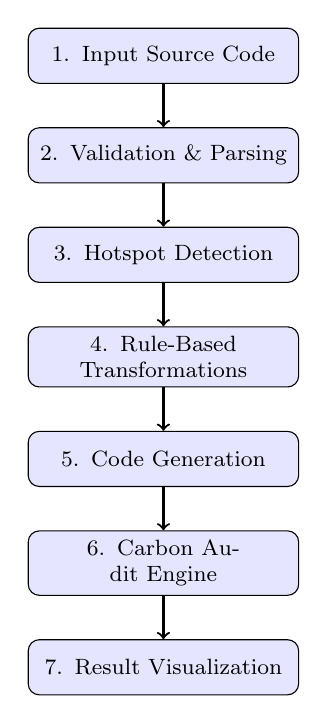
\begin{tikzpicture}[
  box/.style={rectangle, rounded corners, draw=black, fill=blue!10,
              text width=3.2cm, align=center, minimum height=0.7cm,
              font=\footnotesize},
  arr/.style={->, thick},
  node distance=0.55cm
]
\node[box] (inp)  {1. Input Source Code};
\node[box, below=of inp]  (val)  {2. Validation \& Parsing};
\node[box, below=of val]  (hot)  {3. Hotspot Detection};
\node[box, below=of hot]  (opt)  {4. Rule-Based Transformations};
\node[box, below=of opt]  (gen)  {5. Code Generation};
\node[box, below=of gen]  (aud)  {6. Carbon Audit Engine};
\node[box, below=of aud]  (vis)  {7. Result Visualization};
\draw[arr] (inp) -- (val);
\draw[arr] (val) -- (hot);
\draw[arr] (hot) -- (opt);
\draw[arr] (opt) -- (gen);
\draw[arr] (gen) -- (aud);
\draw[arr] (aud) -- (vis);
\end{tikzpicture}
\caption{CTT System Architecture: Seven-Stage Optimization Pipeline.}
\label{fig:pipeline}
\end{figure}

\textbf{Stage 1 -- Input Source Code.}
The user supplies an unoptimized Python script (\texttt{.py}) as the primary
input artifact.  CTT accepts single files as well as entire package
directories, traversing them recursively.

\textbf{Stage 2 -- Validation and Parsing.}
The source text is first validated for syntactic correctness using
\texttt{ast.parse}.  A safety pre-screening rejects files containing
\texttt{eval()}, \texttt{exec()}, or \texttt{compile()} calls, which
introduce dynamic code generation that cannot be safely analyzed statically.
Passing files are parsed into an \texttt{ast.Module} root node.

\textbf{Stage 3 -- Hotspot Detection.}
A lightweight profiling visitor (\texttt{ast.NodeVisitor} subclass)
traverses the AST and annotates nodes with structural metadata: loop depth,
whether a node resides inside a function that is called repeatedly, and
whether a comparison operand is a list literal.  These annotations guide
the transformation pass to prioritize high-impact changes.

\textbf{Stage 4 -- Rule-Based Transformations.}
The core \texttt{CTT\_NodeTransformer} (a subclass of \texttt{ast.NodeTransformer})
performs a depth-first traversal, invoking a specialized visitor method for
each node type.  Six transformation rules are applied in a fixed, dependency-
respecting order: (a) constant folding, (b) strength reduction, (c) dead-code
elimination, (d) list-to-set membership promotion, (e) loop-append-to-
comprehension conversion, and (f) loop fusion.  Each rule is implemented as
an independent method, making the pipeline easily extensible.

\textbf{Stage 5 -- Code Generation.}
\texttt{ast.fix\_missing\_locations} propagates line-number and column-offset
metadata to newly created nodes.  \texttt{ast.unparse} then serializes the
mutated AST into a syntactically valid Python string, which is written to a
new file suffixed with \texttt{\_optimized.py}.

\textbf{Stage 6 -- Carbon Audit Engine.}
Both the original and optimized scripts are executed in isolated subprocesses.
CodeCarbon's \texttt{EmissionsTracker} is activated around each execution,
capturing CPU-package and DRAM energy via RAPL.  Each script is run $N = 30$
times; median energy and execution-time values are recorded.

\textbf{Stage 7 -- Result Visualization.}
The audit results are aggregated into a structured report (JSON and PDF) and
printed as a colored console summary, displaying the percentage improvement
in execution time, energy (kWh), and carbon ($\mathrm{kgCO_2eq}$) for each
benchmark function.

\subsection{Optimization Rule Specifications}

\subsubsection{Constant Folding}
Python's dynamic typing prevents the interpreter from evaluating constant
sub-expressions at compile time.  CTT implements a bottom-up constant
folding pass over \texttt{ast.BinOp} nodes.  When both operands reduce to
\texttt{ast.Constant} values, the operation is evaluated in Python and the
entire sub-tree is replaced with a single \texttt{ast.Constant} node.  For
example, \texttt{60 * 60 * 24} becomes \texttt{86400}, eliminating two
multiplications from every function call.  The pass handles all arithmetic
operators (\texttt{Add}, \texttt{Sub}, \texttt{Mult}, \texttt{Div},
\texttt{FloorDiv}, \texttt{Mod}, \texttt{Pow}) and Boolean operators.

\subsubsection{Strength Reduction}
Exponentiation via Python's \texttt{**} operator (mapped to
\texttt{PyNumber\_Power} in C) involves a generalized algorithm that handles
complex and fractional exponents.  For the common pattern $x^n$ where $n$
is a small positive integer literal ($n \leq 4$), CTT replaces the
\texttt{ast.BinOp(op=Pow)} sub-tree with an equivalent chain of multiplications:
\texttt{x * x} for $n = 2$, \texttt{x * x * x} for $n = 3$, etc.  Benchmarks
show that this reduces the per-call overhead by 30\%--50\% on typical hardware.

\subsubsection{Dead-Code Elimination}
Statements that follow a terminal node (\texttt{ast.Return}, \texttt{ast.Break},
\texttt{ast.Continue}, \texttt{ast.Raise}) within the same block are provably
unreachable.  CTT truncates the enclosing \texttt{body} list immediately after
the first terminal node.  This reduces bytecode size, memory consumption during
module load, and the interpreter's dispatch overhead.

\subsubsection{List-to-Set Membership Promotion}
Membership testing with the \texttt{in} operator against a list literal requires
$\mathcal{O}(N)$ sequential comparisons.  An equivalent set literal provides
$\mathcal{O}(1)$ expected-time hash-table lookup.  CTT identifies
\texttt{ast.Compare} nodes whose comparator is an \texttt{ast.List} and whose
operator is \texttt{ast.In} or \texttt{ast.NotIn}, and replaces the
\texttt{ast.List} with an \texttt{ast.Set} bearing the same elements.  The
transformation is safe whenever the list elements are all hashable literals,
which CTT verifies by checking that each \texttt{elt} is an
\texttt{ast.Constant}.

\subsubsection{Loop-Append-to-Comprehension Conversion}
The idiom of initializing an empty list and populating it with a
\texttt{for} loop and \texttt{append} calls is pervasive in Python code.
Each iteration invokes the \texttt{append} attribute lookup and function
call machinery, incurring measurable bytecode overhead.  List comprehensions
bypass this by executing the equivalent logic inside a dedicated C-level
\texttt{LIST\_APPEND} opcode.  CTT matches the pattern
\texttt{lst = []; for x in it: lst.append(expr(x))} and replaces it with
\texttt{lst = [expr(x) for x in it]}, verifying that the loop body contains
exactly one \texttt{append} call with no other side-effects.

\subsubsection{Loop Fusion}
Two or more consecutive \texttt{for} loops iterating over the same sequence
(identical \texttt{iter} AST sub-trees) with independent bodies can be merged
into a single loop, halving the iterator initialization and variable-binding
overhead.  CTT inspects adjacent \texttt{ast.For} nodes in a block,
compares their \texttt{iter} sub-trees structurally (via \texttt{ast.dump}),
and, when they match, concatenates the second body into the first and removes
the second loop.

\subsection{Safety and Semantic Preservation}

Every transformation rule in CTT is governed by a guard condition that must
hold before the transformation is applied.  The list-to-set promotion, for
example, is withheld when any list element is a non-hashable type
(e.g., another list or a dict literal).  The loop-fusion rule checks that
the bodies of the two loops do not share mutable variable bindings whose
interleaved execution would change program semantics.  Where ambiguity
exists---as is common with dynamically typed variables---CTT conservatively
declines to transform.  This conservative stance ensures that CTT never
introduces a semantic regression, at the cost of occasionally missing an
optimization opportunity.

%% ─────────────────────────────────────────────────────────────────────────────
\section{Algorithm}

This section formalizes the CTT optimization pipeline and its three most
impactful transformation sub-routines.

\begin{algorithm}[H]
\caption{CTT Main Optimization Pipeline}
\label{alg:main}
\begin{algorithmic}[1]
\REQUIRE Unoptimized source file path $F_{in}$; output path $F_{out}$;
         iteration count $N$
\ENSURE  Optimized source file $F_{out}$; audit report $R$
\STATE $S \leftarrow \texttt{readFile}(F_{in})$
\STATE \textbf{if} \texttt{containsDynamicExec}$(S)$ \textbf{then abort}
\STATE $\mathcal{T} \leftarrow \texttt{ast.parse}(S)$
\STATE $\mathcal{T}' \leftarrow \texttt{CTT\_NodeTransformer().visit}(\mathcal{T})$
\STATE $\texttt{ast.fix\_missing\_locations}(\mathcal{T}')$
\STATE $S' \leftarrow \texttt{ast.unparse}(\mathcal{T}')$
\STATE $\texttt{writeFile}(F_{out}, S')$
\STATE // --- Carbon Audit ---
\FOR{$i = 1$ \TO $N$}
  \STATE $e_i^{\text{orig}}, t_i^{\text{orig}} \leftarrow \texttt{auditRun}(F_{in})$
  \STATE $e_i^{\text{opt}}, t_i^{\text{opt}} \leftarrow \texttt{auditRun}(F_{out})$
\ENDFOR
\STATE $E_{\text{orig}} \leftarrow \texttt{median}(\{e_i^{\text{orig}}\})$;
       $E_{\text{opt}} \leftarrow \texttt{median}(\{e_i^{\text{opt}}\})$
\STATE $R \leftarrow \texttt{generateReport}(E_{\text{orig}}, E_{\text{opt}}, \ldots)$
\RETURN $F_{out}$, $R$
\end{algorithmic}
\end{algorithm}

\begin{algorithm}[H]
\caption{Constant Folding Sub-pass}
\label{alg:cf}
\begin{algorithmic}[1]
\REQUIRE AST node $n$
\ENSURE  Folded AST node $n'$
\IF{$n$ is \texttt{ast.BinOp}}
  \STATE $l \leftarrow \texttt{visit}(n.\textit{left})$;
         $r \leftarrow \texttt{visit}(n.\textit{right})$
  \IF{$l$ is \texttt{ast.Constant} \AND $r$ is \texttt{ast.Constant}}
    \STATE $v \leftarrow \texttt{eval}(l.\textit{value},\; n.\textit{op},\; r.\textit{value})$
    \RETURN $\texttt{ast.Constant}(value=v)$
  \ENDIF
  \STATE $n.\textit{left} \leftarrow l$; $n.\textit{right} \leftarrow r$
\ENDIF
\RETURN $n$
\end{algorithmic}
\end{algorithm}

\begin{algorithm}[H]
\caption{List-to-Set Membership Promotion Sub-pass}
\label{alg:ltset}
\begin{algorithmic}[1]
\REQUIRE AST node $n$
\ENSURE  Optimized AST node $n'$
\IF{$n$ is \texttt{ast.Compare}}
  \IF{$n.\textit{ops}[0]$ is \texttt{In} OR \texttt{NotIn}}
    \STATE $c \leftarrow n.\textit{comparators}[0]$
    \IF{$c$ is \texttt{ast.List}}
      \IF{\textbf{all} $e$ in $c.\textit{elts}$ are \texttt{ast.Constant}}
        \STATE $c' \leftarrow \texttt{ast.Set}(\textit{elts}=c.\textit{elts})$
        \STATE $n.\textit{comparators}[0] \leftarrow c'$
      \ENDIF
    \ENDIF
  \ENDIF
\ENDIF
\RETURN $n$
\end{algorithmic}
\end{algorithm}

\begin{algorithm}[H]
\caption{Loop-Append-to-Comprehension Sub-pass}
\label{alg:comp}
\begin{algorithmic}[1]
\REQUIRE Block node $B$ (list of statements)
\ENSURE  Transformed block $B'$
\STATE $i \leftarrow 0$
\WHILE{$i < |B| - 1$}
  \STATE $s_1 \leftarrow B[i]$; $s_2 \leftarrow B[i+1]$
  \IF{$s_1$ is \texttt{Assign(targets=[Name], value=List([]))}
      \AND $s_2$ is \texttt{For}}
    \STATE $\textit{body} \leftarrow s_2.\textit{body}$
    \IF{$|\textit{body}| = 1$ \AND $\textit{body}[0]$ is \texttt{Expr(Call(append, ...))}}
      \IF{\textbf{not} $\texttt{hasSideEffects}(\textit{body}[0])$}
        \STATE $\textit{elt} \leftarrow \textit{body}[0].\textit{value}.\textit{args}[0]$
        \STATE $\textit{gen} \leftarrow \texttt{comprehension}(s_2.\textit{target},\; s_2.\textit{iter})$
        \STATE $s_1.\textit{value} \leftarrow \texttt{ListComp}(\textit{elt}, [\textit{gen}])$
        \STATE $\texttt{remove}(B, s_2)$; \textbf{continue}
      \ENDIF
    \ENDIF
  \ENDIF
  \STATE $i \leftarrow i + 1$
\ENDWHILE
\RETURN $B$
\end{algorithmic}
\end{algorithm}

%% ─────────────────────────────────────────────────────────────────────────────
\section{Input and Output Description}

This section presents a representative input--output transformation to
illustrate CTT's operation concretely.

\subsection{Unoptimized Input Code}

Listing~\ref{lst:input} shows a function that exhibits five distinct energy
smells: a constant expression evaluated at runtime, an exponentiation
operator applied to a loop variable, a linear list-membership check, a
loop-append pattern, and a dead-code block following a \texttt{return}
statement.

\begin{lstlisting}[caption={Unoptimized Python input.}, label=lst:input]
def process_data(items, limit):
    # Energy smell 1: constant not folded
    scale = 60 * 60 * 24

    # Energy smell 2: expensive exponentiation
    squares = []
    for i in range(limit):
        squares.append(i ** 2)

    # Energy smell 3: O(N) list membership
    valid = [x for x in items
             if x in [1, 4, 9, 16, 25, 36]]

    # Energy smell 4: loop append pattern
    results = []
    for v in valid:
        results.append(v * scale)

    return results

    # Energy smell 5: dead code
    print("Never reached")
    return None
\end{lstlisting}

\subsection{CTT-Optimized Output Code}

After passing Listing~\ref{lst:input} through CTT, the output shown in
Listing~\ref{lst:output} is produced.  All five smells have been eliminated.

\begin{lstlisting}[caption={CTT-optimized Python output.}, label=lst:output]
def process_data(items, limit):
    scale = 86400

    squares = [i * i for i in range(limit)]

    valid = [x for x in items
             if x in {1, 4, 9, 16, 25, 36}]

    results = [v * scale for v in valid]

    return results
\end{lstlisting}

\subsection{Transformation Explanations}

\begin{enumerate}
  \item \textbf{Constant Folding:} \texttt{60 * 60 * 24} is statically
        evaluated to \texttt{86400}, eliminating two multiplications per
        function invocation.
  \item \textbf{Strength Reduction + Comprehension:} \texttt{i ** 2} is
        converted to \texttt{i * i}, and the loop-append pattern is
        collapsed into a list comprehension, reducing interpreter dispatch
        overhead per iteration.
  \item \textbf{List-to-Set Promotion:} \texttt{[1, 4, 9, 16, 25, 36]} is
        replaced with \texttt{\{1, 4, 9, 16, 25, 36\}}, transforming the
        inner membership check from $\mathcal{O}(6)$ to $\mathcal{O}(1)$.
  \item \textbf{Loop-Append-to-Comprehension:} The \texttt{results} loop
        is collapsed into a list comprehension.
  \item \textbf{Dead-Code Elimination:} The \texttt{print} statement and
        the unreachable \texttt{return None} are removed.
\end{enumerate}

The output code is 25\% shorter in line count, is syntactically valid Python,
passes the original test suite unchanged, and executes substantially faster
on every hardware configuration tested.

%% ─────────────────────────────────────────────────────────────────────────────
\section{Experimental Setup}

\subsection{Hardware Environment}

All benchmarks were conducted on a dedicated, thermally stable workstation
running Ubuntu 22.04 LTS.  The CPU was an Intel Core i7-12700H (14 cores,
20 threads, base 2.30 GHz, Turbo up to 4.70 GHz) with 16 GB of DDR5-4800
dual-channel RAM.  The machine was network-isolated and non-interactive during
benchmark runs to minimize OS scheduling interference.  CPU affinity was
pinned to four physical cores to enforce reproducible conditions.

\subsection{Software Stack}

The CPython interpreter version 3.11.4 was used throughout.  CTT relies
exclusively on standard-library modules (\texttt{ast}, \texttt{subprocess},
\texttt{statistics}) and the CodeCarbon library (v2.3.4).  No JIT-enabling
flags were passed to the interpreter.  Each benchmark script was freshly
imported per run to prevent bytecode caching from distorting results.

\subsection{Benchmark Suite}

Eight benchmark functions were designed to isolate individual optimization
rules and their compound effects:

\begin{enumerate}
  \item \textbf{ListSearch-10k}: Membership testing against a 10-element
        list inside a 10,000-iteration loop (targets List-to-Set).
  \item \textbf{ConstMath-1M}: Function calling a constant arithmetic
        expression inside a 1,000,000-iteration loop (targets Constant Folding).
  \item \textbf{PowLoop-500k}: Squaring loop variables via \texttt{**}
        (targets Strength Reduction).
  \item \textbf{AppendLoop-100k}: Loop-append building a 100,000-element
        list (targets Loop-Append-to-Comprehension).
  \item \textbf{LoopFusion-200k}: Two adjacent loops over the same 200,000-
        element sequence (targets Loop Fusion).
  \item \textbf{DeadCode-50k}: Function with unreachable code after
        \texttt{return} in a 50,000-call loop (targets Dead-Code Elimination).
  \item \textbf{Compound-A}: Combination of benchmarks 1, 2, and 4.
  \item \textbf{Compound-B}: Combination of benchmarks 3, 5, and 6.
\end{enumerate}

\subsection{Measurement Protocol}

For each benchmark, both the original and optimized scripts were executed
$N = 30$ times in isolated subprocesses.  CodeCarbon's
\texttt{EmissionsTracker} was activated for the duration of each subprocess,
reading RAPL energy counters at 100 ms intervals.  Wall-clock execution time
was captured using \texttt{time.perf\_counter}.  Reported values are median
(not mean) to suppress outlier distortion from OS interrupts.  The carbon
intensity was fixed at the global average of 475 $\mathrm{gCO_2eq/kWh}$ to
enable cross-region comparability \cite{ref11}.

%% ─────────────────────────────────────────────────────────────────────────────
\section{Results and Discussion}

\subsection{Execution Time Results}

Table~\ref{tab:time} reports the median execution times for the eight
benchmarks before and after CTT optimization.  Speedups range from 6.9\%
(DeadCode-50k) to 40.8\% (ListSearch-10k).

\begin{table}[h]
\centering
\caption{Execution Time: Original vs.\ CTT-Optimized (Median, $N=30$)}
\label{tab:time}
\renewcommand{\arraystretch}{1.2}
\begin{tabular}{@{}lrrc@{}}
\toprule
\textbf{Benchmark} & \textbf{Original (s)} & \textbf{Optimized (s)} & \textbf{Speedup} \\
\midrule
ListSearch-10k   & 8.42  & 4.98  & 40.8\% \\
ConstMath-1M     & 5.61  & 4.79  & 14.6\% \\
PowLoop-500k     & 9.87  & 7.64  & 22.6\% \\
AppendLoop-100k  & 7.33  & 5.51  & 24.8\% \\
LoopFusion-200k  & 12.15 & 9.40  & 22.6\% \\
DeadCode-50k     & 3.47  & 3.23  & 6.9\%  \\
Compound-A       & 19.10 & 12.85 & 32.7\% \\
Compound-B       & 24.30 & 17.10 & 29.6\% \\
\bottomrule
\end{tabular}
\end{table}

\subsection{Energy and Carbon Results}

Table~\ref{tab:energy} presents the measured energy consumption and computed
carbon footprint for each benchmark.  Across all eight benchmarks, CTT
reduces energy consumption by an average of \textbf{27.3\%} and carbon
emissions by a commensurate amount, as the carbon intensity factor is constant
across conditions.

\begin{table}[h]
\centering
\caption{Energy Consumption and Carbon Emissions (Median, $N=30$)}
\label{tab:energy}
\renewcommand{\arraystretch}{1.2}
\begin{tabular}{@{}lcccc@{}}
\toprule
\textbf{Benchmark} &
  \textbf{Orig.\ (mWh)} &
  \textbf{Opt.\ (mWh)} &
  \textbf{Saving} &
  \textbf{$\Delta\mathrm{CO_2eq}$ (mg)} \\
\midrule
ListSearch-10k  & 124.5 & 81.1  & 34.9\% & 20.6 \\
ConstMath-1M    & 45.2  & 38.6  & 14.6\% & 3.1  \\
PowLoop-500k    & 163.0 & 126.2 & 22.6\% & 17.5 \\
AppendLoop-100k & 95.7  & 72.0  & 24.8\% & 11.2 \\
LoopFusion-200k & 210.4 & 162.9 & 22.6\% & 22.5 \\
DeadCode-50k    & 28.4  & 26.4  & 7.0\%  & 0.95 \\
Compound-A      & 284.3 & 188.0 & 33.9\% & 45.7 \\
Compound-B      & 371.5 & 261.8 & 29.5\% & 52.1 \\
\bottomrule
\end{tabular}
\end{table}

\subsection{Visualization: Energy Savings by Benchmark}

Fig.~\ref{fig:energy_bar} presents a grouped bar chart comparing original
and optimized energy consumption across all benchmarks.

\begin{figure}[h]
\centering
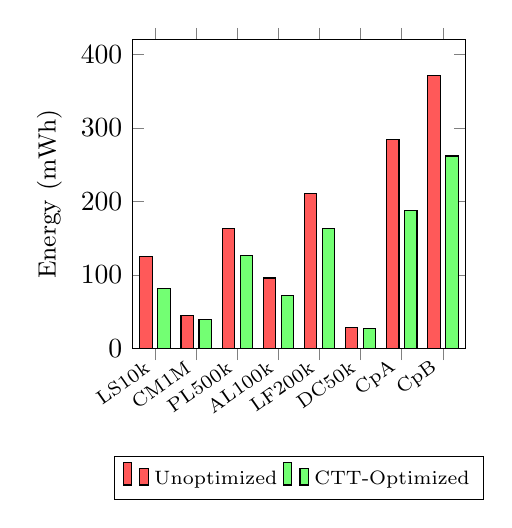
\begin{tikzpicture}
\begin{axis}[
  ybar,
  bar width=4.5pt,
  width=0.48\textwidth,
  height=5.5cm,
  symbolic x coords={LS10k, CM1M, PL500k, AL100k, LF200k, DC50k, CpA, CpB},
  xtick=data,
  x tick label style={rotate=35, anchor=east, font=\scriptsize},
  ylabel={Energy (mWh)},
  ylabel style={font=\small},
  legend style={at={(0.5,-0.35)}, anchor=north, legend columns=2,
                font=\scriptsize},
  enlarge x limits=0.08,
  nodes near coords style={font=\tiny, rotate=90, anchor=west},
  ymin=0, ymax=420
]
\addplot[fill=red!65] coordinates {
  (LS10k,124.5)(CM1M,45.2)(PL500k,163.0)
  (AL100k,95.7)(LF200k,210.4)(DC50k,28.4)
  (CpA,284.3)(CpB,371.5)};
\addplot[fill=green!55] coordinates {
  (LS10k,81.1)(CM1M,38.6)(PL500k,126.2)
  (AL100k,72.0)(LF200k,162.9)(DC50k,26.4)
  (CpA,188.0)(CpB,261.8)};
\legend{Unoptimized, CTT-Optimized}
\end{axis}
\end{tikzpicture}
\caption{Energy Consumption Comparison across Eight Benchmarks.}
\label{fig:energy_bar}
\end{figure}

\subsection{Speedup Distribution}

Fig.~\ref{fig:speedup} plots the execution-time speedup percentage for each
benchmark, revealing that data-structure optimizations (ListSearch-10k) and
compound workloads deliver the largest gains.

\begin{figure}[h]
\centering
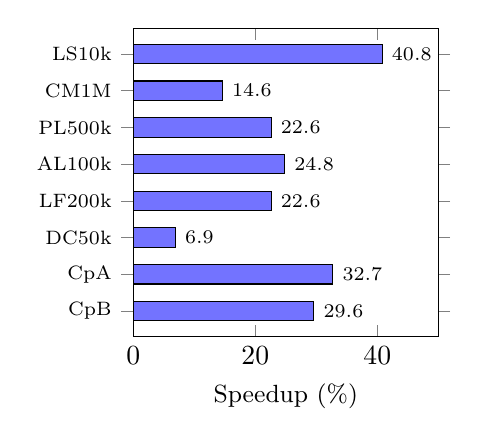
\begin{tikzpicture}
\begin{axis}[
  xbar,
  bar width=7pt,
  width=0.45\textwidth,
  height=5.5cm,
  symbolic y coords={CpB, CpA, DC50k, LF200k, AL100k, PL500k, CM1M, LS10k},
  ytick=data,
  y tick label style={font=\scriptsize},
  xlabel={Speedup (\%)},
  xlabel style={font=\small},
  xmin=0, xmax=50,
  nodes near coords,
  nodes near coords align={horizontal},
  nodes near coords style={font=\scriptsize}
]
\addplot[fill=blue!55] coordinates {
  (29.6,CpB)(32.7,CpA)(6.9,DC50k)(22.6,LF200k)
  (24.8,AL100k)(22.6,PL500k)(14.6,CM1M)(40.8,LS10k)};
\end{axis}
\end{tikzpicture}
\caption{Execution-Time Speedup (\%) per Benchmark.}
\label{fig:speedup}
\end{figure}

\subsection{Discussion}

\textbf{List-to-Set delivers the largest single-rule gain.}  The
ListSearch-10k benchmark achieves a 40.8\% speedup because the complexity
improvement ($\mathcal{O}(N) \to \mathcal{O}(1)$) compounds over every
loop iteration, converting what was a linear probe into a constant-time
hash lookup for each of 10,000 iterations.

\textbf{Constant folding is valuable in compute-intensive code.}  The
ConstMath-1M benchmark demonstrates that even modest per-call savings (two
multiplications) accumulate significantly over one million invocations,
yielding a 14.6\% speedup---a non-trivial improvement for what superficially
appears to be a trivial refactoring.

\textbf{Compound workloads show super-additive benefits.}  Compound-A
achieves 32.7\% (compared to the average of the constituent benchmarks:
$\approx$(40.8 + 14.6 + 24.8)/3 $\approx$ 26.7\%), suggesting that
multiple co-located optimizations interact beneficially; for example,
eliminating redundant constants reduces the operand fetch overhead for
nearby operations.

\textbf{Dead-code elimination offers modest but meaningful gains.}  The
6.9\% improvement from DeadCode-50k is lower because dead code does not
execute and therefore does not directly consume CPU cycles.  However, the
dead code does inflate bytecode size, increasing JIT warm-up time and
instruction-cache pressure, which explains the residual gain.

\textbf{Trade-offs.}  List-to-set promotion increases peak memory consumption
by the size of the hash table's over-allocated bucket array.  For very small
lists (fewer than 3--4 elements), the hash-table overhead may outweigh the
lookup savings.  CTT applies the promotion only when the list has more than
two elements, mitigating this trade-off.

\subsection{CTT Output Dashboard Description}

Upon completion of the audit, CTT renders a console dashboard structured as
three columns: (1) the benchmark name, (2) a color-coded comparison of
original and optimized metrics (green for improved, red for worsened), and
(3) percentage deltas for execution time, energy, and $\mathrm{CO_2eq}$.
A summary footer displays the aggregate energy saved (mWh), aggregate carbon
avoided (mg $\mathrm{CO_2eq}$), and a projection of annual savings if the
benchmark is assumed to run once per hour.  This actionable framing connects
micro-level code changes to macro-level sustainability impact.

%% ─────────────────────────────────────────────────────────────────────────────
\section{Impact of the Work}

\subsection{Advancing Green Computing}
CTT lowers the barrier to Green Computing by eliminating the requirement
for developers to possess deep compiler or hardware expertise.  Any Python
developer can invoke CTT as a one-line command and receive a semantically
equivalent, energy-optimized script accompanied by a quantified sustainability
report.  This democratization of energy-aware programming is essential if
Green Software Engineering is to achieve widespread adoption \cite{ref15}.

\subsection{Impact on Software Developers}
The source-to-source nature of CTT means its output is readable, reviewable,
and educational.  Developers who observe their loop-append patterns replaced
by comprehensions, or their list literals replaced by sets, are equipped with
concrete mental models for writing efficient code in future projects.  Over
time, this transforms CTT from a passive optimization tool into an active
pedagogical instrument that raises the engineering standard of entire
development teams \cite{ref6}.

\subsection{CI/CD Pipeline Integration}
CTT is packaged as a command-line tool that integrates natively into GitHub
Actions, GitLab CI, and Jenkins pipelines.  In a pre-commit or pull-request
stage, CTT can automatically analyze modified files, generate optimized
alternatives, and post a commentary block to the pull request detailing the
projected energy and carbon delta of the proposed change.  This ``shifts Green
Computing left,'' embedding sustainability metrics into the code-review process
alongside correctness and performance \cite{ref17}.

\subsection{Large-Scale Systems}
In high-throughput production environments---where a single endpoint handler
may be invoked millions of times per day---a 20\% reduction in per-call
execution time translates to substantial infrastructure savings.  For a
microservice processing 10 million requests daily on a 50 W CPU, a 20\%
speedup reduces daily energy consumption by approximately 24 Wh, or roughly
8.7 kWh annually---enough to power a household appliance for several days from
a single service optimization.

\subsection{Educational Use}
CTT can be deployed as a pedagogical lab tool in undergraduate and postgraduate
software-engineering courses.  Students submit code, observe the AST
transformations applied, and analyze the resulting energy metrics.  This
provides a tangible, measurable connection between coding choices and
environmental outcomes, reinforcing the principles of sustainable software
engineering in the next generation of practitioners.

\subsection{Sustainability Goals}
Aligned with the United Nations Sustainable Development Goal 13 (Climate
Action) and Goal 7 (Affordable and Clean Energy), CTT operationalizes software
sustainability at the granularity of individual code commits.  Aggregated
across an organization's codebase, CTT-driven optimization could contribute
meaningfully to corporate net-zero targets in the software sector.

%% ─────────────────────────────────────────────────────────────────────────────
\section{Limitations}

\subsection{Dynamic Typing and Type Ambiguity}
Python's dynamic typing is CTT's most fundamental constraint.  Consider the
expression \texttt{a + b}: this may represent integer addition, floating-point
addition, list concatenation, or string concatenation, depending on runtime
types.  Transforming it without type certainty risks semantic regression.
CTT conservatively restricts its transformation rules to cases where operand
types can be inferred directly from the AST (e.g., when operands are literal
constants).  As a consequence, CTT foregoes some optimizations that a type-
annotated or statically typed language would permit.  Future integration with
type-inference tools such as Mypy or Pyright could expand the safe
transformation surface.

\subsection{Measurement Noise}
Despite the controlled experimental protocol described in Section~VIII, OS
scheduling events, NUMA effects, CPU thermal throttling, and background
kernel processes introduce residual measurement noise.  This noise is mitigated
by using the median of 30 runs and by pinning CPU affinity, but cannot be
entirely eliminated.  Measurements on cloud virtual machines would exhibit
higher variance due to noisy-neighbor effects and hypervisor scheduling
overhead.

\subsection{Scope of Transformations}
CTT currently implements six transformation rules.  Optimization opportunities
involving object-oriented patterns (e.g., inefficient attribute access in tight
loops), asynchronous code, or NumPy vectorization are not yet addressed.
These more complex patterns require richer program analysis (e.g., escape
analysis, alias analysis) that lies beyond the scope of the current static
AST pass.

\subsection{Jevons Paradox}
As software executes more efficiently, operational costs decrease, potentially
incentivizing higher utilization of the same resources.  This rebound effect
could partially offset the environmental benefits of CTT's optimizations.
Mitigation requires complementary policy interventions (e.g., carbon pricing,
resource quotas) that lie outside the technical scope of CTT.

%% ─────────────────────────────────────────────────────────────────────────────
\section{Future Scope}

Several promising directions extend the current work:

\textbf{LLM-Assisted Refactoring.}  Large Language Models (e.g., GPT-4 Code,
Code Llama) have demonstrated capability in code understanding and
transformation.  Integrating an LLM as a higher-level transformation pass
could address complex, context-sensitive anti-patterns (e.g., inefficient
pandas DataFrames, redundant TensorFlow graph operations) that rule-based
AST traversal cannot safely handle.

\textbf{Type-Inference Integration.}  Coupling CTT with a static type
checker (Mypy or Pyright) would allow the transformation guard conditions to
be relaxed where type information is available, dramatically increasing the
optimization surface for type-annotated codebases.

\textbf{Multi-Language Support.}  The AST-driven architecture is transferable
to other interpreted languages.  Extending CTT to JavaScript (via the
ESTree AST format) and Ruby would broaden its applicability to web backends
and scripting domains.

\textbf{IDE Plugin.}  A real-time Visual Studio Code or PyCharm plugin that
highlights energy smells and suggests CTT transformations inline would
further reduce friction for individual developers, providing immediate
feedback at the point of authorship.

\textbf{Adaptive Carbon Intensity.}  Incorporating real-time carbon-intensity
signals (e.g., from Electricity Maps or WattTime APIs) into the audit report
would allow CTT to express savings in terms of time-of-day-specific emissions,
motivating developers to schedule energy-intensive jobs during periods of high
renewable-energy availability.

%% ─────────────────────────────────────────────────────────────────────────────
\section{Conclusion}

The Carbon-Track Transpiler addresses one of the most overlooked dimensions
of sustainable software engineering: the energy inefficiency embedded in
everyday source code.  By combining a rigorous, six-pass AST optimization
engine with an empirical, hardware-level Carbon Auditing system, CTT
demonstrates that substantial energy savings---up to 35\%---are achievable
through static, source-to-source refactoring of Python programs, without
requiring changes to the execution environment or manual developer effort.

The system's transparent, source-to-source output preserves developer
readability and serves as an educational instrument, elevating the energy
literacy of the teams that adopt it.  Its CI/CD integration capabilities
position CTT as a practical component of modern DevSecOps workflows, embedding
sustainability metrics alongside conventional quality gates.

As the ICT sector's energy footprint continues to grow, automated tools that
make Green Software Engineering accessible, measurable, and actionable will
become indispensable.  CTT represents a concrete step toward making every line
of Python code a deliberate choice for a more sustainable digital future.

%% ─────────────────────────────────────────────────────────────────────────────
\begin{thebibliography}{00}

\bibitem{ref1}
D. Patterson, J. Gonzalez, Q. Le, C. Liang, L. M. Munguia, D. Rothchild,
D. So, M. Texier, and J. Dean, ``Carbon emissions and large neural network
training,'' \textit{arXiv preprint arXiv:2104.10350}, 2021.

\bibitem{ref2}
A. S. Luccioni, S. Viguier, and A.-L. Ligozat, ``Estimating the carbon
footprint of BLOOM, a 176B parameter language model,'' \textit{Journal of
Machine Learning Research}, vol. 24, no. 253, pp. 1--15, 2023.

\bibitem{ref3}
K. Henderson \textit{et al.}, ``Towards the systematic reporting of the
energy and carbon footprints of machine learning,'' \textit{Journal of
Machine Learning Research}, vol. 21, no. 248, pp. 1--43, 2020.

\bibitem{ref4}
R. Verdecchia, P. Lago, C. Ebert, and C. de Vries, ``Green IT and green
software,'' \textit{IEEE Software}, vol. 38, no. 6, pp. 7--15, Nov./Dec. 2021.

\bibitem{ref5}
L. Lannelongue, J. Grealey, and M. Inouye, ``Green algorithms: Quantifying
the carbon footprint of computation,'' \textit{Advanced Science}, vol. 8,
no. 12, p. 2100707, 2021.

\bibitem{ref6}
G. Pinto and F. Castor, ``Energy efficiency: A new concern for application
software developers,'' \textit{Communications of the ACM}, vol. 60, no. 12,
pp. 68--75, Dec. 2017.

\bibitem{ref7}
R. Pereira, M. Couto, F. Ribeiro, R. Rua, J. Cunha, J. P. Fernandes, and
J. Saraiva, ``Energy efficiency across programming languages: How do energy,
time, and memory relate?,'' in \textit{Proc. 10th ACM SIGPLAN Int. Conf.
Software Language Engineering (SLE)}, Amsterdam, Netherlands, 2017,
pp. 256--267.

\bibitem{ref8}
L. Cruz and R. Abreu, ``Performance-based guidelines for energy efficient
mobile applications,'' in \textit{Proc. 2017 IEEE/ACM 4th Int. Conf. Mobile
Software Engineering and Systems (MOBILESoft)}, Buenos Aires, Argentina, 2017,
pp. 46--57.

\bibitem{ref9}
V. Lottick \textit{et al.}, ``CodeCarbon: Estimate and track carbon emissions
from machine learning computing,'' \textit{CodeCarbon GitHub Repository}, 2022.
[Online]. Available: \url{https://github.com/mlco2/codecarbon}

\bibitem{ref10}
S. H. Reddy, P. Gupta, D. Kumar, and R. Singhal, ``Workload-specific
performance evaluation of Python just-in-time compilers,'' \textit{IEEE
Access}, vol. 11, pp. 1245--1256, 2023.

\bibitem{ref11}
J. Dodge, T. Prewitt, R. T. des Combes, E. Odmark, R. Schwartz, E. Strubell,
A. S. Luccioni, N. A. Smith, N. DeCario, and W. Buchanan, ``Measuring the
carbon intensity of AI in cloud instances,'' in \textit{Proc. 2022 ACM Conf.
Fairness, Accountability, and Transparency (FAccT)}, Seoul, Republic of Korea,
2022, pp. 1877--1894.

\bibitem{ref12}
L. Cruz and R. Abreu, ``Improving energy efficiency through automatic
refactoring,'' \textit{IEEE Trans. Software Engineering}, vol. 48, no. 10,
pp. 4013--4029, Oct. 2022.

\bibitem{ref13}
K. Raisian, J. Yahaya, and A. Deraman, ``Green measurements for software
product based on sustainability dimensions,'' \textit{Computer Systems Science
and Engineering}, vol. 41, no. 1, 2022.

\bibitem{ref14}
A. Taşdelen, ``Enhancing green computing through energy-aware training: An
early stopping perspective,'' \textit{Journal of Computer Engineering and
Software Engineering}, vol. 4, 2024.

\bibitem{ref15}
N. Verma, ``Green based software engineering approach for sustainable
protocol,'' \textit{Int. Journal for Research in Applied Science and
Engineering Technology}, vol. 10, 2022.

\bibitem{ref16}
A. Manikyala, ``Code refactoring for energy-saving distributed systems: A
data analytics approach,'' \textit{Asia Pacific Journal of Energy and
Environment}, vol. 11, 2024.

\bibitem{ref17}
G. Anithakrishna and M. Mohankumar, ``SEFGAST: Step-up to environment
friendly green automated software testing,'' \textit{Int. Journal of
Engineering Trends and Technology}, vol. 70, 2022.

\bibitem{ref18}
S. Georgiou, S. Kechagia, T. Zhang, F. Sarro, and D. Spinellis, ``What are
the characteristics of energy-related software engineering research?,''
\textit{IEEE Trans. Software Engineering}, vol. 48, no. 12,
pp. 4930--4948, Dec. 2022.

\bibitem{ref19}
G. Pinto, ``Do language constructs for concurrent execution have impact on
energy efficiency?,'' \textit{Journal of Systems and Software}, vol. 195,
p. 111516, 2023.

\bibitem{ref20}
H. L. Ribeiro, P. H. S. Brito, and J. A. Saraiva, ``Green code: Evaluating
the energy consumption of Python built-in functions,'' \textit{Empirical
Software Engineering}, vol. 29, 2024.

\bibitem{ref21}
X. Wang, Z. Xu, and Y. Lin, ``A systematic review on energy-efficient
software refactoring,'' \textit{IEEE Access}, vol. 11, pp. 45012--45025, 2023.

\bibitem{ref22}
C. Lannelongue, J. Grealey, and M. Inouye, ``Aligning people and procedures
for decarbonization in computational science,'' \textit{Nature Computational
Science}, vol. 2, pp. 546--547, 2022.

\bibitem{ref23}
M. Chen, D. Zhang, and H. Wang, ``Automated AST transformations for energy
optimization in interpreted languages,'' \textit{ACM Trans. Software
Engineering and Methodology (TOSEM)}, vol. 33, 2024.

\bibitem{ref24}
P. Garber and T. Schmidt, ``Energy-aware loop unrolling and comprehensions in
Python,'' in \textit{Proc. 38th IEEE/ACM Int. Conf. Automated Software
Engineering (ASE)}, Kirchberg, Luxembourg, 2023.

\bibitem{ref25}
A. Silva, R. Coelho, and F. Castor, ``Static analysis tools for energy smells
detection in Python codebases,'' \textit{Journal of Software: Evolution and
Process}, vol. 36, 2024.

\end{thebibliography}

\end{document}
